\documentclass[10pt ]{article}
\usepackage{bbm}
\usepackage{times}
\usepackage{epsfig}
\usepackage{graphicx}
\usepackage{amsmath}
\usepackage{amssymb}
\usepackage{amsthm}
\usepackage{hyperref}
\usepackage{soul}
\usepackage[]{algorithm2e}

\hypersetup{
    colorlinks=true,
    linkcolor=blue,
    filecolor=magenta,      
    urlcolor=cyan,
}
\urlstyle{same}

\DeclareMathOperator*{\argmaxA}{arg\,max}
\DeclareMathOperator*{\argminA}{arg\,min}

\newtheorem{example}{Example}
\newtheorem{thm}{Theorem}
\newtheorem{corol}{Corollary}
\newtheorem{obs}{Observation}
\newtheorem{fact}{Fact}
\newtheorem{mydef}{Definition}
\newtheorem{lem}{Lemma}
\newtheorem{prop}{Proposition}

\usepackage{tikz}
\usepackage{soul}
\usetikzlibrary{shapes.misc, positioning, shapes.geometric, arrows}
%\usepackage[a4paper,margin=1cm,landscape]{geometry}
\usetikzlibrary{positioning,shapes,shadows}


\tikzstyle{conv2d} = [rectangle, rounded corners, minimum width=4cm, minimum height=1cm,text centered, draw=black, fill=green!30]
\tikzstyle{bn} = [rectangle, rounded corners, minimum width=4cm, minimum height=1cm,text centered, draw=black, fill=red!30]
\tikzstyle{relu} = [rectangle, rounded corners, minimum width=4cm, minimum height=1cm,text centered, draw=black, fill=blue!30]
\tikzstyle{add} = [circle, radius=1cm,text centered, draw=black]
\tikzstyle{arrow} = [thick,->,>=stealth]
\tikzstyle{downsample} = [rectangle, minimum width=6cm, minimum height=4cm,text centered, draw=black, fill=yellow!30]
\tikzstyle{maxpool} = [rectangle, rounded corners, minimum width=4cm, minimum height=1cm,text centered, draw=black, fill=gray!30]

\tikzstyle{btds} = [rectangle, rounded corners, minimum width=4cm, minimum height=1cm,text centered, draw=black, fill=orange!30]

\tikzstyle{btnods} = [rectangle, rounded corners, minimum width=4cm, minimum height=1cm,text centered, draw=black, fill=violet!30]

\tikzstyle{block} = [draw, fill=white, rectangle, 
    minimum height=3em, minimum width=6em]

\tikzstyle{boostingblock} = [draw, fill=white, rectangle, 
    minimum height=2em, minimum width=4em]

\tikzstyle{bigblock} = [draw,  rectangle, 
    minimum height=15em, minimum width=20em]
    
\def\ttx{1.4}

\setcounter{page}{1}
\begin{document}

\title{Statistical learning theory by Robert Schapire}

\author{Mohsen Kiskani}

\maketitle

I happened to see the following video series by Robert Schapire on Youtube,
\begin{enumerate}
\item \url{https://www.youtube.com/watch?v=3wbLr-NnIKI}
\item \url{https://www.youtube.com/watch?v=bjzMmXgM0OU}
\item \url{https://www.youtube.com/watch?v=YyhpS5ltuKA}
\item \url{https://www.youtube.com/watch?v=yvdq0CE0l5g}
\item \url{https://www.youtube.com/watch?v=Hm4I05LH9ns}
\end{enumerate}
In the following, I bring a summary of these videos. 

\section*{Lecture 1}
The following rules are enough for learning and we need them.
\begin{itemize}
\item Enough data
\item Fit to training data (consistent or few mistakes)
\item A rule that is as simple as possible. 
\end{itemize}
There is a trade-off between the second and the third rules which we want to understand. 

Some notations:
\begin{itemize}
\item \textbf{Instance} $x$ belonging to an \textbf{instance space} $X$, ($x \in X$) is assumes to be coming from a \textbf{target distribution} $D$ which is fixed but unknown. We do not know this distribution and we do not have any assumptions on this distribution so we have a \textbf{distribution free} learning algorithm. It is assumed that each training or test example $x_i$ comes from distribution $D$ and they are i.i.d.
\item \textbf{label/class} $\{0,1\}$. There is some function $c:X \to \{0,1\}$ that maps instances to labels. This labeling function is called a \textbf{concept}. Therefore, for each instance $x$ we have a label $c(x)$. Our goal is to learn the concept $c$ or an approximation of it. Usually we assume that the concept $c$ is coming from a \textbf{concept class} $\mathcal{C}$.
\item \textbf{hypothesis} A hypothesis $h:X\to \{0,1\}$ is a prediction rule that tries to predict the concept. To measure how good is the hypothesis we measure the probability of choosing a test instance that is misclassified. This is called the \textbf{error} or \textbf{generalization error},
\begin{align}
\mathrm{err}_D(h) \triangleq \mathrm{Pr}_{x \sim D}\left[ h(x) \neq c(x)\right].
\end{align}
We want this error to be small $\mathrm{err}_D(h)\le  \epsilon$ or in other words, we want it to be \textbf{approximately correct}. But there is a bit of problem here. Since the samples are selected randomly, there is always a small chance that the training data 
is a terrible training set. For instance, if we are learning handwritten characters, there is a small chance that our training dataset only contains vowels. So it will not be able to work properly on the general dataset. So we allow the learning algorithm to fail in this scenario but we need to control the probability of it's failing over the choice of the training sample. Hence, we want the probability of error of the output hypothesis (which is random because it depends on the training sample) to be
\begin{align}
\mathrm{Pr} \left[ \mathrm{err}_D(h) \le \epsilon \right] \ge 1-\delta,
\end{align}
where the probability is taken over the choice of the training sample. This method is called \textbf{Probably Approximately Correct} or \textbf{PAC} learning. 
\item A \textbf{learning algorithm} $\mathcal{A}$ is an algorithm that takes $m$ instances along with their labels i.e. $\{(x_1, c(x_1)), (x_2, c(x_2)), \dots, (x_m, c(x_m))$ and comes up with the hypothesis $h$. 
\item Concept class $\mathcal{C}$ is \textbf{PAC learnable} if there exists a learning algorithm $\mathcal{A}$ such that for every concept $c \in \mathcal{C}$ and for any target distribution $D$ and for every $\epsilon >0$ and for every $\delta > 0 $, algorithm $\mathcal{A}$ takes $m = \mathrm{Poly}(1/\epsilon, 1/\delta, ...)$ random examples $x_i$ from $D$ and outputs a hypothesis $h$ such that 
\begin{align}
\mathrm{Pr} \left[ \mathrm{err}_D(h) \le \epsilon \right] \ge 1-\delta,
\end{align}
where 
\begin{align}
\mathrm{err}_D(h) \triangleq \mathrm{Pr}_{x \sim D}\left[ h(x) \neq c(x)\right].
\end{align}
Notice that as $\epsilon$ and $\delta$ get smaller and smaller, we need to have more training data. Hence, we allow $m$ to be a polynomial in $1/\epsilon$ and $1/\delta$ along with other stuff. 
\item Sometimes it is helpful to assume that the hypothesis comes from a specific \textbf{hypothesis class} $\mathcal{H}$ which is a different class than $\mathcal{C}$ and the learning algorithms outputs from that hypothesis space. If the learning algorithm is supposed to only output hypotheses from $\mathcal{H}$, then we say that a concept class $\mathcal{C}$ is \textbf{PAC learnable by $\mathcal{H}$} if the above holds for $h \in \mathcal{H}$.
\end{itemize}
Is this kind of learning possible? The domain $\mathcal{H}$ is typically gigantic, even infinite, and we are trying to find  from a small polynomial size sample a rule which is correct on almost all of the examples!
\begin{example}{\em
\label{example_positive_half_lines}
Assume that your domain $X = [0,1]$ is the set of all real numbers between 0 and 1. The instances are just points on the real line between 0 and 1. The concepts are simple threshold functions between 0 and 1. If an instance is above the threshold, then it is labeled positive and if it less than the threshold it is labeled negative. We know that there is a threshold function which is consistent with these examples but we don't know which particular function it is. We call these concepts {\em positive half lines} which constitute our concept class. So the concept class $\mathcal{C}$ is the set of all positive half lines. Given data of this kind, we basically need to choose a threshold between the rightmost negative sample and the leftmost positive sample and call that our hypothesis. The hypothesis class in this case is the same as the concept class. One choice (not necessarily the best) is to choose the threshold as the leftmost positive example, $b$, and let $h(x) = 1$ if $x \ge b$ and  $h(x) = 0$ if $x < b$. Now, the interesting question is, is this algorithm PAC? To show that it is PAC, we need to bound the probability of error. An error happens if we get a new positive sample that is less than $b$ but more than the true threshold $c$. 

For any $\epsilon >0$ assume that the region between $c$ and $c+\epsilon$ is called $S$ where $0 \le c$ and $c + \epsilon \le 1$. For any training example, if even one positive training example $x_i$ falls in $S$, then the hypothesis have to be either at $x_i$ or to the left. Then we will have to have $h$ falling into the region $S$. So error happens if none of the positive training examples fall within $S$. This means that we will have  
\begin{align}
\mathrm{Pr} \left[ \mathrm{err}_D(h) > \epsilon \right] &\le  \mathrm{Pr} \left[ \mathrm{No ~positive~ x_i ~ falls ~in ~S} \right] \le  \mathrm{Pr} \left[ \forall i \in \{1,\dots,m\}~ x_i \notin S \right] \nonumber \\
&=\prod_{i=1}^m \mathrm{Pr} \left[ x_i \notin S \right] = (1-\epsilon)^m \le  e^{-m\epsilon}.
\end{align}
Hence, we should have 
\begin{align}
m \ge \frac{\log(1/\delta)}{\epsilon}
\end{align}
}
\end{example}

\section*{Lecture 2}
To simplify the PAC learning problem, we assume that the hypothesis space is finite $|\mathcal{H}| < \infty$. We can prove the following theorem
\begin{thm}
{\em 
If algorithm $\mathcal{A}$ finds a hypothesis $h_{\mathcal{A}} \in \mathcal{H}$ which is consistent with $m$ random training examples from distribution $D$ where 
\begin{align}
m \ge \frac{1}{\epsilon} \left( \log(|\mathcal{H}|) + \log(\frac{1}{
\delta})\right)
\end{align}
then 
\begin{align}
\mathrm{Pr} \left[ \mathrm{err}_D(h_{\mathcal{A}}) \ge \epsilon\right] \le \delta.
\end{align}
Equivalently, if we are given $m$ examples, then with probability of at least $1-\delta$ we have 
\begin{align}
\mathrm{err}_D(h_{\mathcal{A}}) \le \frac{1}{m} \left( \log(|\mathcal{H}|) + \log(\frac{1}{
\delta})\right)
\end{align}
}
\label{thm_pac_finite_1}
\end{thm}

The notion of \textbf{consistent} in the above theorem is different from the notion of consistency in statistics and simply means that the hypothesis and the concept values agree on the sample data.
In this bound, $ \log(|\mathcal{H}|) $ shows a measure of the complexity of the hypothesis space.  Further, this bounds captures the three conditions we need for learning. We can have an accurate classifier which means that $\epsilon$ is small, by having enough data, $m$ large enough and we can bound the complexity i.e. $\log(|\mathcal{H}|)$ in this case. Instead of proving the above theorem, we will prove a slightly stronger result as follows.

\begin{thm}
{\em 
Assume $m$ is given such that 
\begin{align}
m \ge \frac{1}{\epsilon} \left( \log(|\mathcal{H}|) + \log(\frac{1}{
\delta})\right)
\end{align}
then with probability of at least $1-\delta$, for every $h \in \mathcal{H}$, if $h$ is consistent with the training samples we have
\begin{align}
 \mathrm{err}_D(h) \le \epsilon 
 \label{eq_h_e_good}
\end{align}
}
\label{thm_pac_finite_2}
\end{thm}
Note that Theorem \ref{thm_pac_finite_2} is stronger than Theorem \ref{thm_pac_finite_1} and if proved, directly proves Theorem \ref{thm_pac_finite_1}. To summarize the notation, if for some $h$, equation \eqref{eq_h_e_good} is valid, the hypothesis $h$ is called \textbf{$\epsilon$-good} and otherwise, it is called \textbf{$\epsilon$-bad.} To prove Theorem \ref{thm_pac_finite_2} we want to prove that 
\begin{align}
\mathrm{Pr}\left[ \forall h \in \mathcal{H}: ~ h ~\mathrm{consistent} \Rightarrow h ~\mathrm{is}~ \epsilon-\mathrm{good}\right] \ge 1 - \delta
\end{align}
or equivalently 
\begin{align}
\mathrm{Pr}\left[ \exists h \in \mathcal{H}: ~ h ~\mathrm{consistent} ~\mathrm{and}~ h ~\mathrm{is}~ \epsilon-\mathrm{bad}\right] \le  \delta
\end{align}
In the following, we will prove Theorem \ref{thm_pac_finite_2}.
\begin{proof}
Define 
\begin{align}
\mathcal{B} = \{h \in \mathcal{H} \mid h ~\mathrm{is}~ \epsilon-\textrm{bad}\}
\end{align}
Hence, using the union bound we have 
\begin{align}
&\mathrm{Pr}\left[ \exists h \in \mathcal{H}: ~ h ~\mathrm{consistent} ~\mathrm{and}~ h ~\mathrm{is}~ \epsilon-\mathrm{bad}\right] = \mathrm{Pr}\left[ \exists h \in \mathcal{B} \mid h ~\mathrm{is~ consistent}~ \right] \nonumber \\
&\le \sum_{h \in \mathcal{B}} \mathrm{Pr} \left[ h ~\mathrm{is~ consistent} \right] = \sum_{h \in \mathcal{B}} \prod_{i=1}^m \mathrm{Pr} \left[ h(x_i) = c(x_i)\right] \nonumber \\
&\le \sum_{h \in \mathcal{B}}  (1-\epsilon)^m = |\mathcal{B}| (1-\epsilon)^m \le |\mathcal{H}| (1-\epsilon)^m \le |\mathcal{H}| e^{-\epsilon m} \le \delta 
\end{align}
\end{proof}

A problem with Theorems \ref{thm_pac_finite_1} and \ref{thm_pac_finite_2} is that they require the hypothesis to be consistent. Also, we want to extend these ideas to the case of infinite hypothesis space. We know based on our previous example that PAC learning is possible for some infinite classes. Now, we want to study this problem in more detail and see what is it about these infinite classes that makes PAC learning possible.  As a first step, let's look at our previous example. For this example, assuming that we have $m$ training points, then we can observe at most $m+1$ possible behaviours (label assignments) depending on where the threshold would fall along the [0, 1] line. This is much smaller than the total number of $2^m$ possible behaviours (label assignments). In these nice cases, we are only getting a polynomial number of behaviours on any training set. This is kind of the intuition that we were hoping to find. Given a sample of $m$ examples, we can somehow treat these labeling or these labelings as forming a kind of effective hypothesis space and work with that hypothesis space rather than the full hypothesis space.  We can make this more formal. 

For any set $S \triangleq \{x_1, \dots, x_m\}$ of training examples we can write down the behaviour of any particular hypothesis on that sample as 
\begin{align}
\Pi_{\mathcal{H}}(S) \triangleq \{\langle h(x_1), \dots, h(x_m) \rangle \mid h \in \mathcal{H}\}.
\end{align}
Then we can look at the cardinality of this set for any sample of size $S$. We want to find the maximum cardinality of these sets over all possible sets of size $m$. With a little bit of overloading we can define the \textbf{growth function} as 
\begin{align}
\Pi_{\mathcal{H}}(m) = \max_{|S|=m} |\Pi_{\mathcal{H}}(S)|.
\end{align}
We hope to find a bound similar to the one that we found for finite hypotheses and apply it somehow to these labeling to treat them as kind of an effective hypothesis space. This is indeed possible and we can prove the following theorem.
\begin{thm}
{\em
Given $m$ training examples with probability $1-\delta$, for every $h \in \mathcal{H}$, if $h$ is consistent, then 
\begin{align}
\mathrm{err}_D(h) \le  O \left( \frac{\log\left(2\Pi_{\mathcal{H}}(m)\right) + \log\left(\frac{1}{\delta}\right)}{m}\right)
\end{align}
}\label{thm_infinite_H}
\end{thm}
Notice that in nice cases when the growth function $\Pi_{\mathcal{H}}(m)$ is a polynomial i.e. $\Pi_{\mathcal{H}}(m) = O(m^d)$, we have 
\begin{align}
\mathrm{err}_D(h) \le  O \left( \frac{d\log\left(m\right) + \log\left(\frac{1}{\delta}\right)}{m}\right)
\label{eq_vc_dim_err_bnd}
\end{align}
which is a nice bound that goes to zero with $m$.

\begin{obs}{\em 
Note that we started with a question about probabilistic learnability where all the data is random and the test data is also random and we wanted to prove something probabilistically about performance. This seems to be a question that is all about probability but what Theorems \ref{thm_pac_finite_1} and \ref{thm_infinite_H} tell us is that all that matters is combinatorial properties of the hypothesis space. In other words,
\begin{itemize}
\item If you are working with a finite hypothesis space and you are able to find a finite hypothesis, to show that it has low error and it is a PAC algorithm, all you have to do is to just count how many hypotheses there are.
\item When you are working with infinite hypothesis spaces, again the question boils down to a question that involves counting, combinatorial properties of the hypothesis space. 
\end{itemize}
}
\end{obs}
\begin{prop}{\em
It can be proved that the growth function can only take two cases and there are no other cases. Either 
\begin{align}
\Pi_{\mathcal{H}}(m) & = 2^m  \\
&\mathrm{or} \nonumber \\
\Pi_{\mathcal{H}}(m) & = O(m^d)
\end{align}
We either have the worst possible case, or the nice cases. What's more, is that this dichotomy of the two cases exactly corresponds to when PAC learning is possible subject to all our previous assumptions (regardless of computation complexity). 
}\label{prop_dichotomy_growth}
\end{prop}

It turns out that the constant $d$ is a special combinatorial parameter which is called the \textbf{VC-Dimension}.

\begin{mydef}
{\em 
If we have a sample $S$ of size $m$ points, then this sample is \textbf{shattered} by a hypothesis space $\mathcal{H}$, if all behaviours are possible. In other words, 
\begin{align}
|\Pi_{\mathcal{H}}(S)| =  2^m.
\end{align}
The \textbf{VC-Dimension} of a hypothesis class $\mathcal{H}$ is the size of the largest shattered set. 
}
\end{mydef}
\begin{example}
{\em 
If the hypothesis space $\mathcal{H}$ is the class of all intervals, i.e. domain of real numbers. The hypothesis is positive for points inside interval and negative outside the interval. If $m=2$, then a sample space of two points is shattered by $\mathcal{H}$ while if $m=3$, it cannot be shattered by $\mathcal{H}$ because no such hypothesis would allow a negative labeling to the middle point and positive labels to the side points. Hence, the VC dimension of intervals is 2. 
}
\end{example}

A really important class of hypotheses is the set of \textbf{Linear Threshold Functions (LTF)} in $\mathbb{R}^n$ which is a function defined by a hyper-plane and all the points above the hyper-plane are classified positive while all the points under the hyper-plane are classified negative. The VC dimension of this class is $n+1$. If the LTF is forced to go through the origin, then it's VC dimension is just $n$.

If $\mathcal{H}$ is finite, i.e. $|\mathcal{H}| < \infty$, then $\mathrm{VC}(\mathcal{H}) \le \log_2|\mathcal{H}|$ (notice that $\log_2|\mathcal{H}|$ is our earlier complexity measure on finite spaces).

\section*{Lecture 3}
If the VC dimension is infinite, it means that for any $m$, we can get a shattered set of that size. 
\begin{lem}
{\em
\textbf{Sauer's Lemma:} If we have a class of hypotheses $\mathcal{H}$ with finite VC dimension $d$, then the growth function is bounded by 
\begin{align}
\Pi_{\mathcal{H}}(m) \le \sum_{i=0}^m {m \choose i}
\end{align}
}
\end{lem}
\begin{corol}{\em
If we have a class of hypotheses $\mathcal{H}$ with finite VC dimension $d$, and if $1 \le d \le m$, then 
\begin{align}
\Pi_{\mathcal{H}}(m) \le \sum_{i=0}^m {m \choose i} \le \left( \frac{e m }{d} \right)^d
\end{align}
and therefore, $\Pi_{\mathcal{H}}(m) = O(m^d)$ which proves the second scenario in Proposition \ref{prop_dichotomy_growth}. If the VC dimension is infinite this means that for any size $m$, we can find a shattered set which exactly means that all $2^m$ behaviours are possible. This results in the first case in Proposition \ref{prop_dichotomy_growth}. 

}
\end{corol}

The bottom-line from equation \eqref{eq_vc_dim_err_bnd} is that to get a good enough accuracy it's enough to have a number of samples that's linear in the VC dimension. We can also prove that VC dimension is a lower bound on the number of necessary examples required for learning. The basic idea behind proving that is that is the VC dimension is $d$, then all labelings are possible and we need to have $d$ samples to be able to capture all of that. Therefore, VC dimension is both necessary and sufficient. 

How can we extend these results to consider cases where we do not have consistency? There could be many real world scenarios and reasons that we may not have consistency and we want to be able to extend the results to these cases. Up to now, whenever we had an instance $x$, the label would immediately follow through a specific function $c(x)$ but now, we do not assume such a thing and instead we suppose that we have a distribution $D$ which generates samples and labels jointly as $(x, y)$. Now the error is defined as 
\begin{align}
\mathrm{err}_D (h) = \mathrm{Pr}_{(x,y)\sim D} \left[ h(x) \neq y \right]
\end{align}
and we are given a random sample $\{(x_1, y_1),\dots, (x_m,y_m)\}$ and the goal is to find a hypothesis with minimum \textbf{generalization error}
\begin{align}
\min_{h \in \mathcal{H}} \mathrm{err}_D (h). 
\end{align}
The problem is that we do not have direct access to the generalization error but we have a sample. The obvious approach is to just look at the training error of the hypotheses as a proxy to the generalization error and try to minimize that instead. We therefore define the \textbf{training error} or the \textbf{empirical error} or the \textbf{empirical risk} as 
\begin{align}
\widehat{\mathrm{err}}(h) = \frac{1}{m} \sum_{i=1}^m \mathbbm{1}\{h(x_i) \neq y_i\}.
\label{eq_training_err_def}
\end{align}
The idea is to minimize the training error instead of the generalization error. This approach is referred to as \textbf{Empirical Risk Minimization (ERM)}, 
\begin{align}
\hat{h} = \argminA_{h \in \mathcal{H}} \widehat{\mathrm{err}}(h). 
\end{align}
But, how do we show that this simple idea can lead to a hypothesis with a small generalization error? The approach that is generally taken is to try to prove that the training error is close to the generalization error for every hypothesis in the hypothesis space. 

We want to prove that with probability $1-\delta$, for every $h 
\in \mathcal{H}$ we have 
\begin{align}
|\mathrm{err}_D (h) - \widehat{\mathrm{err}}(h)| \le \epsilon.
\end{align}
Notice that the order of quantification is extremely important here. The results wouldn't work if we say something like ``for every $h \in \mathcal{H}$, with probability $1-\delta$'' we in fact want to say that with high probability this result holds for all hypotheses. If we can prove this, then the result shows that the training error is always close to the generalization error. These kinds of results are called \textbf{uniform convergence} results. It is ``uniform'' because we are aiming for a bound which is uniform for all the hypotheses in this space. Notice that ``consistency'' in our previous talks means that the training error $ \widehat{\mathrm{err}}(h)$ be zero which in a uniform convergence sense means that the generalization error is small. But how do we prove these uniform convergence results? 

The easiest case to start with, is to work with a single hypothesis. It has some generalization error and we want to estimate it with the training error. The training error in equation \eqref{eq_training_err_def} is the average of the indicator variables. But notice that 
\begin{align}
 \mathbbm{1}\{h(x_i) \neq y_i\} = \left\{
                \begin{array}{ll}
                1 \qquad \mathrm{with ~probability~} \mathrm{err}_D (h) \\
                  0 \qquad \mathrm{with ~probability~} 1- \mathrm{err}_D (h)
                \end{array}
              \right.
\end{align}
So, to answer this quation, to show that $ \widehat{\mathrm{err}}(h)$ converges to $ \mathrm{err}_D (h)$, we just need to think about coin flopping. How fast does the average of the coin flops converges to the bias of the coin? We can attack this in many ways but a popular form is to use the Chernoff bound. 

\begin{lem}
{\em 
\textbf{Hoeffding's inequality:} We have $m$ i.i.d random variables $Z_i \in [0,1]$,  and let $p = \mathbb{E}[Z_i]$ and let
\begin{align}
\hat{p} = \frac{1}{m} \sum_{i=1}^m Z_i,
\end{align}
then 
\begin{align}
\mathrm{Pr} [\hat{p} \ge p + \epsilon]  \le e^{-2m\epsilon^2}.
\end{align}
}
\end{lem}

\begin{lem}
{\em 
\textbf{McDiarmid's inequality:} Suppose that $f(z_1,\dots,z_m)$ is a real-valued function and suppose that changing $z_i$ only changes $f$ by at most $c_i$. In other words, $\forall z_1,\dots,z_i,\dots,z_m, z_i^{\prime}$
\begin{align}
|f(z_1,\dots,z_i,\dots,z_m) - f(z_1,\dots,z_i^{\prime},\dots,z_m)| \le c_i, 
\end{align}
and if $Z_1,\dots,Z_m$ are independent random variables (not necessarily identically distributed). Then, 
\begin{align}
\mathrm{Pr} \left[ f(Z_1,\dots,Z_m) \ge \mathbb{E}[f(Z_1,\dots,Z_m)]  +\epsilon \right] \le \exp \left( \frac{-2 \epsilon^2}{\sum_{i=1}^m c_i^2}\right)
\end{align}
}\end{lem}

%To prove the desired result using the McDiarmid's inequality, it is enough to 
\begin{obs}{\em
If we choose random variables $Z_i \in [0,1]$ and $c_i = \frac{1}{m}$ and 
\begin{align}
f(Z_1,\dots,Z_m) = \frac{1}{m} \sum_{i=1}^m Z_i,
\end{align}
then McDiarmid's inequality becomes the Hoeffding's inequality. 
}\end{obs}

Now, back to our learning problem, we will use Hoeffding'd inequality with $Z_i = \mathbbm{1} \{h(x_i) \neq y_i\}$. Then, as discussed before,  $p=\mathbb{E} [ Z_i ] = \mathrm{err}_D(h)$ and $\hat{p} = \widehat{\mathrm{err}}(h)$ and therefore
\begin{align}
\mathrm{Pr} \left[| \mathrm{err}_D(h) -   \widehat{\mathrm{err}}(h) | \ge \epsilon \right] \le 2 e^{-2\epsilon^2 m}.
\end{align}
This is good because it proves that the training error $\widehat{\mathrm{err}}(h)$ is indeed close to the generalization error $\mathrm{err}_D(h)$ for the case of a single hypothesis. We will now consider the case of finite hypothesis spaces, i.e. $|\mathcal{H}|<\infty$ and we want to prove uniform convergence on that. We can use the union bound to get 
\begin{align}
\mathrm{Pr} \left[ \exists h \in \mathcal{H} \mid | \mathrm{err}_D(h) -   \widehat{\mathrm{err}}(h) | \ge \epsilon \right] \le 2 |\mathcal{H}| e^{-2\epsilon^2 m}.
\label{eq_hoedding_finite}
\end{align}
This bound tells us that given $m$ training examples, with probability at least $1-\delta$ equation \eqref{eq_hoedding_finite} is not true which means that 
\begin{align}
\forall h \in \mathcal{H}: \quad | \mathrm{err}_D(h) -   \widehat{\mathrm{err}}(h) | < O \left( \sqrt{\frac{\log(|\mathcal{H}|) + \log(\frac{1}{\delta})}{m}}\right)
\end{align}
Which can be rewritten as 
\begin{align}
\forall h \in \mathcal{H}: \quad \mathrm{err}_D(h) \le  \widehat{\mathrm{err}}(h)  + O \left( \sqrt{\frac{\log(|\mathcal{H}|) + \log(\frac{1}{\delta})}{m}}\right).
\label{eq_bound_training_err_gen_err}
\end{align}
\begin{obs}{\em
Equation \eqref{eq_bound_training_err_gen_err} tells us that given a certain amount of data,  if we find a hypothesis with a certain training error, then it's generalization error will be at most equal to the training error plus an additional term that depends on the number of training examples and the log of the size of the hypothesis space which is the complexity term. This bounds clearly ties together the bounds that we were talking about, i.e. how well we fit the data, $\widehat{\mathrm{err}}(h)$, how much data we have, $m$, and the complexity of the classifier that we are working with $|\mathcal{H}|$. This kind of bound also makes predictions about how generalization error will be effected by the complexity of the hypotheses that we are working with. Figure \ref{fig_tradeof_complexity} shows how the training and generalization errors change with hypothesis complexity. As can be seen from this picture, as the model complexity increases, training error reduces and because of that, initially the generalization error reduces up to a certain point where it is overwhelmed by the second term which includes the square root of the model complexity. From this point \textbf{overfitting} starts to happen.
\begin{figure}[ht]
\centering
 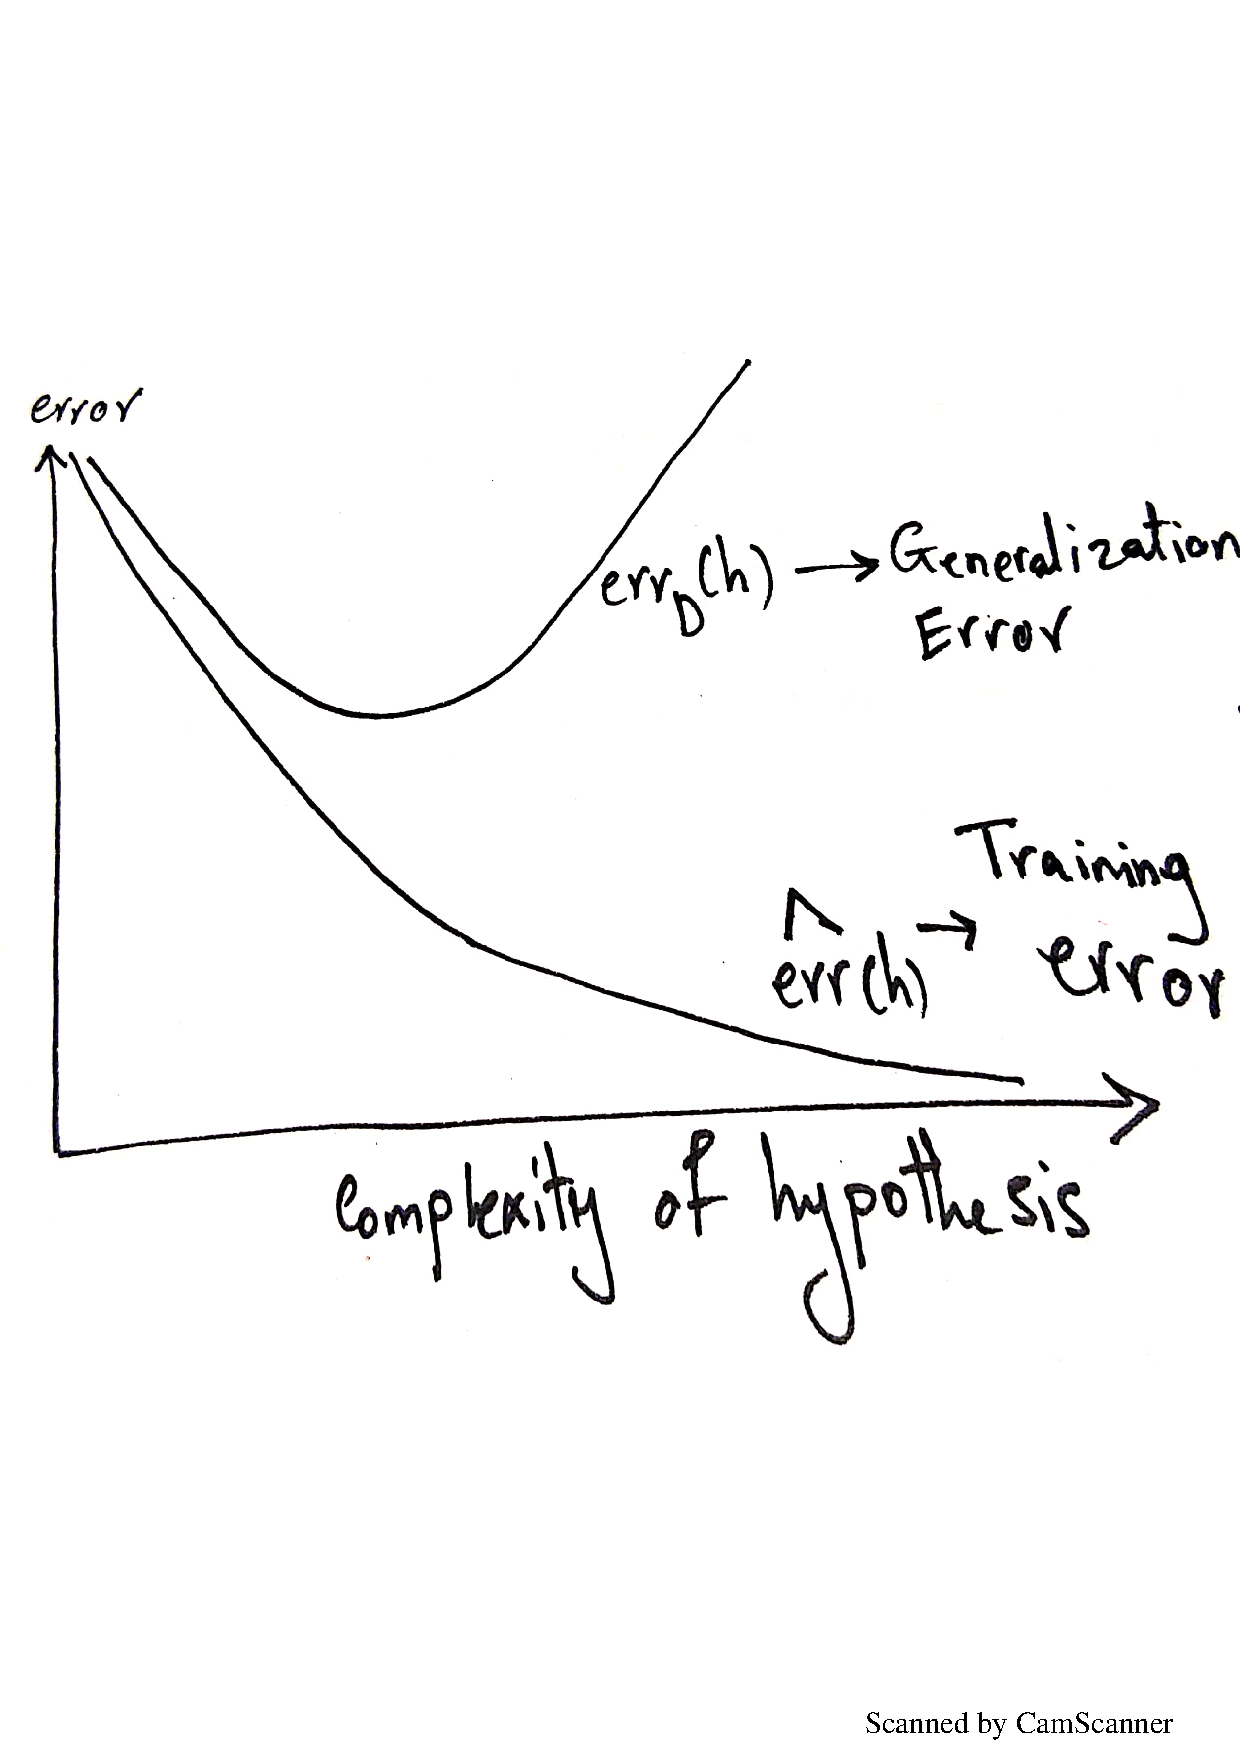
\includegraphics[height=0.5\textwidth]{overfitting.pdf} 
 \caption{Plot of error versus hypothesis complexity}
 \label{fig_tradeof_complexity}
\end{figure}
}
\end{obs}
\begin{obs}
{\em 
The previous bound with consistency does not have the square root and is a better bound. Also, when we have consistency the training error is 0. 
}
\end{obs}

What if the choice of hypothesis space has infinite cardinality? We will introduce another complexity measure and technique for proving uniform convergence results. This complexity measure subsumes all the previous measures that we discussed before. Suppose that we have a labeled sample $S = \{(x_1, y_1),\dots,(x_m,y_m)\}$ where $y_i \in \{-1, +1\}$ and $h ~:~ X \to  \{-1, +1\}$. The basic question is that if we have this particular hypothesis, how well does it fit this sample. If we use the training error we have 
\begin{align}
\widehat{\mathrm{err}}(h) &= \frac{1}{m} \sum_{i=1}^m \mathbbm{1}\{h(x_i) \neq y_i \} = \frac{1}{m} \sum_{i=1}^m \left( \frac{1-y_i h(x_i)}{2} \right) \nonumber \\
&= \frac{1}{2} - \frac{1}{2} \left( \frac{1}{m} \sum_{i=1}^m y_i h(x_i)\right).
\end{align}
Therefore, for a specific hypothesis $h$ it makes sense to use terms like $\sum_{i=1}^m y_i h(x_i)$ to measure how good a hypothesis, $h$ is. What if now we have a class of hypotheses $\mathcal{H}$ and we want to see how well this class of hypotheses $\mathcal{H}$ is to measure the data? To measure how good $\mathcal{H}$ is we look at the best hypothesis in $\mathcal{H}$ and we measure how well it is. Therefore, in this case we need to look at 
\begin{align}
\max_{h \in \mathcal{H}}  \frac{1}{m} \sum_{i=1}^m y_i h(x_i)
\label{eq_measure_new}
\end{align}
as a measure of goodness of the space $\mathcal{H}$. Up to now, everything is defined in a standard way but now to extend this measure and get a more useful measure, we need to see how well the hypotheses in the hypothesis space can fit to noise. We will therefore define the \textbf{Rademacher random variable} as 
\begin{align}
\sigma_i = \left\{ \begin{array}{ll}
                   +1 \quad  \mathrm{with~prob~} \frac{1}{2}\\
                   -1 \quad  \mathrm{with~prob~} \frac{1}{2}
                      \end{array}   
                    \right.  
\label{eq_rademacher_var}
\end{align}
and then we will use Rademacher random variables as our labels. We can then use the measure in equation \eqref{eq_measure_new} and take the expected value with respect to the Rademacher random variables to define \textbf{Rademacher complexity} measure as follows 
\begin{align}
\mathbb{E}_{\sigma} \left[ \max_{h \in \mathcal{H}}  \frac{1}{m} \sum_{i=1}^m \sigma_i h(x_i) \right]
\label{eq_measure_new2}
\end{align}
Why does this measure make sense? The answer lies in the fact that if we have an extremely rich hypothesis space, we have a very rich set of hypotheses and we should be able to fit practically anything even if the labels are random so we have a high Rademacher complexity where as if the hypothesis space is constrained we expect it to be much smaller as we cannot find a hypothesis that can fit noise very well. As an example, if the hypothesis space is just consists of a single hypothesis, then the value of Rademacher complexity is zero and if at the opposite extreme $S$ is shattered by the hypothesis space $\mathcal{H}$, then for any labeling there is some $h$ that exactly matches that labeling and so the inside of bracket is always 1 and the Rademacher complexity will become equal to 1. 

\section*{Lecture 4}
We want to prove that with high probability for every hypothesis $h$ in the hypothesis space, $\widehat{\mathrm{err}}(h) $ eventually converged to $\mathrm{err}_{D}$.  We will prove this in a more  abstract setting. In this new setting, we will be working with functions $f: \mathcal{Z} \to \mathbb{R}$ where $f \in \mathcal{F}$ and samples $z_1,\dots,z_m$ come from the sample space $\mathcal{Z}$. We will work with the \textbf{empirical Rademacher complexity} on this abstract setting defined as 
\begin{align}
\widehat{R}_S({\mathcal{F}}) \triangleq \mathbb{E}_{\sigma} \left[ \sup_{f \in \mathcal{F}} \frac{1}{m} \sum_{i=1}^m \sigma_i f(z_i) \right].
\label{eq_def_rademacher}
\end{align}
The reason that we are working with the supremum instead of maximum is that the maximum might not exist in this general setting. We are sometimes interested to work with the \textbf{expected  Rademacher complexity} taken over the sample, defined as  
\begin{align}
\widehat{R}_m({\mathcal{F}})\triangleq \mathbb{E}_{S} \left[ \widehat{R}_S({\mathcal{F}})  \right].
\end{align}
In this general setting, we want to use Rademacher complexity to prove uniform convergence, i.e. 
 \begin{align}
 \forall f \in \mathcal{F}: \quad \widehat{\mathbb{E}}_{S}\left[ f\right] = \frac{1}{m} \sum_{i=1}^m f(z_i) \to \mathbb{E}_{z \sim D} \left[ f(z) \right].
 \end{align}
\begin{thm}
{\em 
If $\mathcal{F}$ is a family functions $f: Z \to [0,1]$ and $S=\{z_1, \dots, z_m\}$ is a sample where $z_i$'s are i.i.d random variables from a distribution $D$, then with probability at least $1-\delta$ we have 
\begin{align}
 \forall f \in \mathcal{F}: \quad \mathbb{E}_{z \sim D} \left[ f(z) \right] &\le 
 \widehat{\mathbb{E}}_{S}\left[ f\right]  + 2 \widehat{R}_S({\mathcal{F}}) + O\left(\sqrt{\frac{\log(\frac{1}{\delta})}{m}} \right) \label{eq_thm_rademacher_1} \\
 \forall f \in \mathcal{F}: \quad \mathbb{E}_{z \sim D} \left[ f(z) \right] &\le 
 \widehat{\mathbb{E}}_{S}\left[ f\right]  + 2 \widehat{R}_m({\mathcal{F}}) + O\left(\sqrt{\frac{\log(\frac{1}{\delta})}{m}} \right) \label{eq_thm_rademacher_2}
\end{align}
}\label{thm_rademacher}
\end{thm}
We can sort of ignore the last term and basically Theorem \ref{thm_rademacher} says that Rademacher complexity is a uniform upper bound on the difference between the true expectation and the empirical average. 
\begin{proof}
Lets define a random variable $\Phi(S)$ as 
\begin{align}
\Phi(S) \triangleq \sup_{f \in \mathcal{F}}  \left( \mathbb{E}_{z \sim D} \left[ f(z) \right] - \widehat{\mathbb{E}}_{S}\left[ f\right] \right).
\label{eq_def_phi_s}
\end{align}
What we really want to find is a bound on $\Phi(S)$. As a first step, we relate $\Phi(S)$ to it's expected value by proving that 
\begin{align}
\Phi(S) \le \mathbb{E}_S \left[ \Phi(S) \right] + O \left( \sqrt{\frac{\log(\frac{1}{\delta})}{m}} \right).
\end{align}
The proof of this is a direct application of the McDiarmid's inequality by showing that if you change one of the $Z_i$'s in the sample, the most that $\Phi(S)$ can change by is $\frac{1}{m}$. We do not go into the details of that proof. 

Secondly, It is ideal for us to be working with the function $\Phi(S)$ on finite samples.  The second empirical expectation term in equation \eqref{eq_def_phi_s} is taken over a finite set of points and it's fine. The first expectation term is however defined by the distribution $D$ over our entire space and is nasty. A very cool idea is to take an expectation like this and replace it with an empirical average. However, we can't use the empirical average on the sample that we already have so we imagine taking a second set of i.i.d samples $S^{\prime} = \{z_1^{\prime}, \dots, z_m^{\prime}\}$ from the same distribution $D$ and taking average on that imaginary sample. This sample $S^{\prime}$ is often called the \textbf{ghost} sample as opposed to the \textbf{real} sample $S$. The idea is to take the empirical average on the ghost sample and use it as a proxy for $\mathbb{E}_{z \sim D} \left[ f(z) \right]$. In fact, we can prove that 
\begin{align}
 \mathbb{E}_S \left[ \Phi(S) \right] &=  \mathbb{E}_S \left[  \sup_{f \in \mathcal{F}}  \left( \mathbb{E}_{z \sim D} \left[ f(z) \right] - \widehat{\mathbb{E}}_{S}\left[ f\right] \right) \right] \nonumber \\
 &\le  \mathbb{E}_{S, S^{\prime}} \left[  \sup_{f \in \mathcal{F}}  \left(  \widehat{\mathbb{E}}_{S^{\prime}}\left[ f\right]  - \widehat{\mathbb{E}}_{S}\left[ f\right] \right) \right]
 \label{eq_second_idea_rademacher_proof}
\end{align}
Thirdly, there is something else that usually goes along with this ghost sampling idea. If you draw i.i.d data and then reshuffle and re-sample, the sampled data is still i.i.d and the distribution will not change. So, along with choosing the ghost sample, we can imagine injecting a certain kind of randomness that we can closely control into this entire process.  This does not change the data at all but it give us a way to prove stuff. We imagine applying this process to these two samples $S$ and $S^{\prime}$. Imagine that we look at each pair $(z_i, z_i^{\prime}) \in S \times S^{\prime}$ and flip a coin and if it is heads then we swap $z_i$ with $z_i^{\prime}$ and $z_i^{\prime}$ with $z_i$. Otherwise, we leave them alone. We do this for all $i=1,2,\dots,m$. Let's call the resulting ``real'' and ``ghost'' samples $T$ and $T^{\prime}$. The distribution of $T$ and $T^{\prime}$ is exactly the same as the distribution of $S$ and $S^{\prime}$. We have 
\begin{align}
 \widehat{\mathbb{E}}_{S^{\prime}}\left[ f\right]  - \widehat{\mathbb{E}}_{S}\left[ f\right]  = \frac{1}{m} \sum_{i=1}^m \left( f(z_i^{\prime}) - f(z_i)  \right)
\end{align}
and 
\begin{align}
 \widehat{\mathbb{E}}_{T^{\prime}}\left[ f\right]  - \widehat{\mathbb{E}}_{T}\left[ f\right]  &= \frac{1}{m} \sum_{i=1}^m 
 \left\{ \begin{array}{ll}
                    f(z_i^{\prime}) - f(z_i) \quad  \mathrm{with~prob~} \frac{1}{2}\\
                    f(z_i) - f(z_i^{\prime}))\quad  \mathrm{with~prob~} \frac{1}{2}
                      \end{array}   
                    \right.    \nonumber \\
               &= \frac{1}{m} \sum_{i=1}^m  \sigma_i \left(  f(z_i^{\prime}) - f(z_i) \right).
\end{align}
To summarize, from \eqref{eq_second_idea_rademacher_proof}, we have 
\begin{align}
 \mathbb{E}_S \left[ \Phi(S) \right] &\le  \mathbb{E}_{S, S^{\prime}, \sigma} \left[  \sup_{f \in \mathcal{F}} \left( \frac{1}{m} \sum_{i=1}^m  \sigma_i \left(  f(z_i^{\prime}) - f(z_i) \right) \right)  \right].
\end{align}
In step four, we want to prove that the right hand side of the above equation is at most twice the Rademacher complexity. To prove this, notice that, 
\begin{align}
 &\mathbb{E}_{S, S^{\prime}, \sigma} \left[  \sup_{f \in \mathcal{F}} \left( \frac{1}{m} \sum_{i=1}^m  \sigma_i \left(  f(z_i^{\prime}) - f(z_i) \right) \right)  \right]  = \nonumber \\
 & \mathbb{E}_{S, S^{\prime}, \sigma} \left[  \sup_{f \in \mathcal{F}} \left( \frac{1}{m} \sum_{i=1}^m  \sigma_i   f(z_i^{\prime}) + \sum_{i=1}^m  (-\sigma_i) f(z_i)  \right)  \right] \le \nonumber \\
 & \mathbb{E}_{S, S^{\prime}, \sigma} \left[  \sup_{f \in \mathcal{F}} \left( \frac{1}{m} \sum_{i=1}^m  \sigma_i   f(z_i^{\prime}) \right) + \sup_{f \in \mathcal{F}} \left( \sum_{i=1}^m  (-\sigma_i) f(z_i)  \right)  \right] = \nonumber \\
 & \mathbb{E}_{S, S^{\prime}, \sigma} \left[  \sup_{f \in \mathcal{F}} \left( \frac{1}{m} \sum_{i=1}^m  \sigma_i   f(z_i^{\prime}) \right) \right] + \mathbb{E}_{S, S^{\prime}, \sigma} \left[ \sup_{f \in \mathcal{F}} \left( \sum_{i=1}^m  (-\sigma_i) f(z_i)  \right)  \right] = \nonumber \\ 
 & \mathbb{E}_{S^{\prime}, \sigma} \left[  \sup_{f \in \mathcal{F}} \left( \frac{1}{m} \sum_{i=1}^m  \sigma_i   f(z_i^{\prime}) \right) \right] + \mathbb{E}_{S,  \sigma} \left[ \sup_{f \in \mathcal{F}} \left( \sum_{i=1}^m  (-\sigma_i) f(z_i)  \right)  \right] = \nonumber \\ 
&\widehat{R}_m({\mathcal{F}}) + \widehat{R}_m({\mathcal{F}}) = 2 \widehat{R}_m({\mathcal{F}})
\end{align}
In step five, now that we have proved equation \eqref{eq_thm_rademacher_1}, how do we prove \eqref{eq_thm_rademacher_2}? We can again use the McDiarmid's inequality to prove this. Notice that the big O constant in equation \eqref{eq_thm_rademacher_1} may not be correct. 
\end{proof}
Our final goal is to bound $\mathrm{err}_D (h) =\mathbb{E}_D \left[ \mathbbm{1} [h(x) \neq y] \right] $ by  $\widehat{\mathrm{err}}(h)=\widehat{\mathbb{E}}_S \left[ \mathbbm{1} [h(x_i) \neq y_i] \right] $ using the above theorem. Hence, for any hypothesis $h$, we want to define 
\begin{align}
l_h(x,y)\triangleq\mathbbm{1} [h(x) \neq y].
\end{align}
and the class of all these functions as 
\begin{align}
\mathcal{L}_{\mathcal{H}} \triangleq  \{l_h(x,y) \mid h \in \mathcal{H} \}.
\label{eq_class_err_fun_defined}
\end{align}
We can then apply Theorem \ref{thm_rademacher} on the class of functions defined in \eqref{eq_class_err_fun_defined}. When we do that, we will get
\begin{align}
\mathrm{err}_D (h)  \le \widehat{\mathrm{err}}(h) + 2 \widehat{R}_S({\mathcal{L}_{\mathcal{H}} }) + O \left(\sqrt{\frac{\log(\frac{1}{\delta})}{m}} \right).
\end{align}
This is not as desirable as we want since we are more interested to work with the Rademacher complexity of the hypothesis space $\mathcal{H}$ insteas of $\mathcal{L}_{\mathcal{H}} $. But fortunately, we can prove that 
\begin{align}
 \widehat{R}_S({\mathcal{L}_{\mathcal{H}} }) = \frac{1}{2} \widehat{R}_S({\mathcal{H}}).
\end{align}
Hence, we only need to bound the Rademacher complexity of the hypothesis space. To do so, we start from the easiest case, i.e. finite hypothesis space $|\mathcal{H}|<\infty$. In this case, the empirical Rademacher complexity on a sample $S$ can be bounded as 
\begin{align}
\widehat{R}_S({\mathcal{H}}) \le \sqrt{\frac{2 \log |\mathcal{H}|}{m}}.
\end{align}
Notice that our favorite hypothesis measure $\log |\mathcal{H}|$
again shows up in the upper bound. We will now focus on the case of infinite hypothesis spaces. 
\begin{obs}{\em 
One beautiful thing that we can notice for the empirical Rademacher complexity in equation \eqref{eq_def_rademacher} is it's dependence only on the sample itself and not the distribution. So we only care about the \emph{behaviour} of hypotheses in this space on the sample itself. 
}
\end{obs}
Earlier, we talked about the behaviours of hypotheses on the sample. For instance, considering Example \ref{example_positive_half_lines}, we can show that if we have $m$ training samples, then depending on where the thresholding happens we can see at most $m+1$ types of behaviours which is significantly lower than the total $2^m$ possible types of behaviours. Since, empirical Rademacher complexity only cares about these types of behaviours, we can define a new finite space $\mathcal{H}^{\prime}$ which includes only one representative from $\mathcal{H}$ for each behaviour on the sample $S$ itself. The cardinality of $\mathcal{H}^{\prime}$ is equal to the cardinality of the set of all behaviours. Now we can replace $\mathcal{H}$ with $\mathcal{H}^{\prime}$ since all that matters is the bahaviour on the sample. We therefore have, 
\begin{align}
\widehat{R}_S({\mathcal{H}}) &= \mathbb{E}_{\sigma} \left[ \sup_{h \in \mathcal{H}} \frac{1}{m} \sum_{i=1}^m \sigma_i h(z_i) \right] \nonumber \\
&=  \mathbb{E}_{\sigma} \left[ \sup_{h \in \mathcal{H}^{\prime}} \frac{1}{m} \sum_{i=1}^m \sigma_i h(z_i) \right] \nonumber \\
&= \widehat{R}_S({\mathcal{H}^{\prime}}) \le \sqrt{\frac{2 \log |\mathcal{H}^{\prime}|}{m}} = \sqrt{\frac{2 \log |\Pi_{\mathcal{H}}(S)|}{m}}. 
\end{align}
If we now use Sauer's lemma we can get a bound based on VC dimension. 

Moving on to the next topic, we will talk about an interesting algorithm that came from study of theory of statistical learning. Remember in PAC learning model, we require that for any distribution, the learning algorithm has to come up with a hypothesis with low generalization error. For any $\epsilon > 0$, if you give the algorithm enough data, it should be able to get error below $\epsilon$. Now, what if we can't do that? What if we have a learning algorithm which is pretty good and can get the error down to like $30\%$ but no matter how much data you give it, it cannot reduce the error further down. Is there a way of taking an algorithm like that and converting it into an algorithm whose error is as low as you want? What if you have an algorithm that is just a little bit better than random guessing, can you convert it into an algorithm with error below one percent or it is impossible?

In \textbf{strong PAC learning} model, we have a learning algorithm and we feed it examples from a distribution $D$ and it outputs a hypothesis $h$ and the requirement is that $\mathrm{err}_D(h) \le  \epsilon$ for all $\epsilon >0$, given enough data. Instead, suppose that we have a reliable way of getting the error below $1/2$, i.e. there exists some  small positive number $\gamma >0$ such that  $\mathrm{err}_D(h) \le  \frac{1}{2}- \gamma$. We call this new model the  \textbf{weak learning} model, and we are interested to know if these two notions are the same? Are they equivalent to each other? 

\section*{Lecture 5}
Strong and weak learnability are the same and we can prove the following theorem. 
\begin{thm}
{\em 
Class $\mathcal{C}$ is strongly learnable if and only if it is weakly learnable. 
}\label{thm_strong_weak_same}
\end{thm}
The forward direction is trivial but for the backward direction, we need to come up with a method that takes an algorithm that weakly learns a class and converts it into and algorithm that strongly learns the class. This shows that when we talk about PAC learning, learning is an all or nothing phenomenon. Either you can learn a concept class all the way, in the sense of being able to get arbitrary high level accuracy or if that's not possible, it means that it is not even weakly learnable. You can't even learn it a little bit better than random guessing. 

Imagine that we have access to a weak learning algorithm $\mathcal{A}$ that can take any examples from any distribution $D$ and produces a hypothesis $h$ that satisfies  $\mathrm{err}_D(h) \le  \frac{1}{2}- \gamma$ for some $\gamma > 0$ as shown in Figure \ref{fig_weak_learner}. The schematic in Figure \ref{fig_weak_learner} shows that we need to feed random examples according to the distribution $D$ to the algorithm and not necessarily the whole distribution $D$.

\begin{figure}
\centering
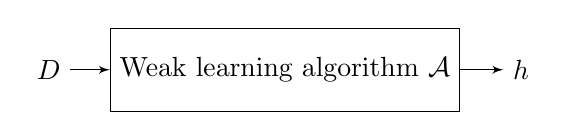
\begin{tikzpicture}[auto, node distance=3cm,>=latex']
    \node [ name=input] {$D$};
    \node [block, right of=input] (algorithm) {Weak learning algorithm $\mathcal{A}$};
    \node [right of=algorithm] (output) {$h$};
    \draw [->] (algorithm) -- node[name=u] {} (output);
    \draw [->] (input) -- node {} (algorithm);
\end{tikzpicture}
\caption{A weak learning algorithm $\mathcal{A}$, takes an example from a distribution $D$ and outputs a hypothesis $h$ such that for some $\gamma >0$, $\mathrm{err}_D(h) \le \frac{1}{2} - \gamma$.}
\label{fig_weak_learner}
\end{figure}

Also, imagine that we are given examples $(x_1,y_1),\dots,(x_m,y_m) \sim \mathcal{D}$ from the true distribution that is generating all the data (assuming that $y_i \in \{-1, +1\}$). We want to find a hypothesis $H$ whose error $\mathrm{err}_{\mathcal{D}}(H)$ is arbitrarily small. An algorithm that can do this is called a \textbf{boosting} algorithm. All we have to do is to work with the learning algorithm and improve it. A natural thing to do is to take this learning algorithm and run it multiple times on our data but if we run the algorithm $\mathcal{A}$ multiple times on the data that we have, we may end up with the same weak hypothesis over and over again. 

Instead, we want to force the weak learning algorithm to do some work and to pay more attention to the hard examples that it keeps misclassifying. The only thing we have to work on is the distribution of the examples that we feed to the learning algorithm. Somehow, we want to feed different examples according to different distributions to the learning algorithm in each one of the boosting algorithm iterations. We have to figure out a way of figuring out these examples from different distributions so that the overall algorithm focuses more on the ``hard'' examples from $\mathcal{D}$. Although the learning algorithm should be able to work with any distribution, in the boosting algorithm we are restricted to working the examples $(x_1,y_1),\dots,(x_m,y_m) \sim \mathcal{D}$ from the true distribution that generates all the data. We will be working only on distributions over this set of examples. The boosting algorithm decides that the real distribution is a distribution that gives weights to the examples in the training set.
\begin{figure}
\centering
\begin{tikzpicture}[auto, >=latex']
     \node [name=originalinput]{$\mathcal{D}$};
     \node [bigblock, right of=originalinput, xshift = 4cm] (algorithm) { };
     \draw [->] (originalinput) -- (algorithm);
     \node [name=finaloutput, right of=algorithm, xshift = 4cm]{$H$};
     \draw [->] (algorithm) -- (finaloutput);
     
     \node [ name=input1, right of=algorithm, xshift = -4cm, yshift = 2cm ] {$D_1$};
     \node [boostingblock, right of=input1, xshift = 2cm] (algorithm1) { $\mathcal{A}$};
     \node [right of=algorithm1, xshift = 2cm] (output1) {$h_1$};
     \draw [->] (algorithm1) -- node[name=u] {} (output1);
     \draw [->] (input1) -- node {} (algorithm1);
     
     \node [ name=input2, below of=input1 , yshift=-0.5cm] {$D_2$};
     \node [boostingblock, right of=input2, xshift = 2cm] (algorithm2) { $\mathcal{A}$};
     \node [right of=algorithm2, xshift = 2cm] (output2) {$h_2$};
     \draw [->] (algorithm2) -- node[name=u] {} (output2);
     \draw [->] (input2) -- node {} (algorithm2);
     
     \node [below of=algorithm2]{$\vdots$};
     \node [ name=input3, below of=input2 , yshift=-1.3cm] {$D_T$};
     \node [boostingblock, right of=input3, xshift = 2cm] (algorithm3) { $\mathcal{A}$};
     \node [right of=algorithm3, xshift = 2cm] (output3) {$h_T$};
     \draw [->] (algorithm3) -- node[name=u] {} (output3);
     \draw [->] (input3) -- node {} (algorithm3);
\end{tikzpicture}
\caption{A schematic representation of the boosting algorithm. A weak learning algorithm $\mathcal{A}$ is run on $T$ iterations over different distributions chosen from $\mathcal{D}$.}
\label{fig_boosting}
\end{figure}
\vspace{0.5cm}
\begin{algorithm}[H]
 \KwData{ Weak learning algorithm $\mathcal{A}$ and  $(x_1,y_1),\dots,(x_m,y_m) \sim \mathcal{D}$.}
 \KwResult{A hypothesis $H$ with arbitrarily small error.}\
 $D_1(i) \gets \frac{1}{m} \quad i=1,\dots,m \quad$ i.e. uniform distribution over the $m$ examples\;
 \For{ $t=1,2,\dots, T$ }{
  \textbf{Run} weak learning algorithm $\mathcal{A}$ on distribution $D_t$ to get weak hypothesis $h_t : \mathbb{X}\to \{-1, +1\}$\;
 \textbf{Compute} the error $\epsilon_t \triangleq \mathrm{err}_{D_t}(h_t)$ where $\epsilon_t = \frac{1}{2}-\gamma_t$ and $0 < \gamma \le \gamma_t$\;
 \textbf{Let}  $\alpha_t \gets \frac{1}{2} \log \left( \frac{1-\epsilon_t}{\epsilon_t}\right)$\;
 \textbf{Construct} \begin{align}
 D_{t+1}(i) = \frac{1}{Z_t}D_t(i) e^{-\alpha_t y_i h_t(x_i)} = \frac{1}{Z_t} D_t(i)  \times \left\{ \begin{array}{ll}
                  e^{-\alpha_t} \quad \mathrm{if~} h_t(x_i) = y_i \\
                  e^{\alpha_t}  ~~\quad \mathrm{if~} h_t(x_i) \neq y_i
                \end{array} \right.
 \nonumber 
\end{align}}\
\textbf{Output} $H(x)$ where $$H(x) = \mathrm{sign} \left( \sum_{t=1}^T \alpha_t h_t(x) \right)$$
 \caption{Pseudo-code for the boosting algorithm \textbf{AdaBoost}}
 \label{alg_boosting}
\end{algorithm}
\vspace{0.5cm}
The main question in boosting is how to create the distributions $D_t$ for $t=1,\dots,T$. Distribution $D_t$ will always be over the examples $(x_1,y_1),\dots,(x_m,y_m)$. So, it can be written as $D_t(x_i, y_i)$ or concisely as $D_t(i)$ for the distribution on the $i^{th}$ example.  The boosting algorithm chooses a distribution in every round. If in round $t$, $h_t(x_i) = y_i$ then we want the algorithm to focus less on that example. So we want to decrease the probability of that event. So we multiply it by a number which is less than one. Otherwise, we increase it's weight by multiplying it by a number greater than one. We choose an exponential multiplier because it makes the math nicer. We also need to normalize the distribution by dividing by the normalization factor $Z_t$. Finally, when computing the final hypothesis $H$, we take the weighted majority vote where the weights are equal to $\alpha_t$'s. 

\begin{thm}
{\em 
Since, $\epsilon_t = \frac{1}{2} -\gamma_t$, we have 
\begin{align}
\widehat{\mathrm{err}}(H) \le \prod_{t=1}^{T} 2 \sqrt{ \epsilon_t (1-\epsilon_t)} = \prod_{t=1}^{T} \sqrt{1-4\gamma_t^2} \le \exp \left( -2 \sum_{t=1}^T \gamma_t^2 \right).
\label{eq_thm_boosting}
\end{align}
If $\forall t$ we have $0<\gamma \le \gamma_t$, then 
\begin{align}
\widehat{\mathrm{err}}(H)  \le e^{-2 \gamma^2 T}
\label{eq_thm_boosting}
\end{align}
This means that so long as $\gamma$ is positive, the training error goes down exponentially fast. 
}\label{thm_boosting_err}
\end{thm}
\begin{proof}
Based on the way that each distribution $D_{t+1}$ is defined and based on the recursion equation in Algorithm \ref{alg_boosting}, we can write, 
\begin{align}
D_{T+1}(i) = \frac{\exp \left( -y_i F(x_i) \right)}{m \prod_{t=1}^T Z_t} 
\label{eq_proof_boosting}
\end{align}
where 
\begin{align}
F(x) \triangleq \sum_{t=1}^T \alpha_t h_t(x)
\end{align}
and $H(x) = \mathrm{sign}\left( F(x) \right)$. Secondly, we show that $\widehat{\mathrm{err}}(H) \le \prod_{t=1}^T Z_t$. To prove this, notice that
\begin{align}
 y \neq H(x) \Leftrightarrow y \neq \mathrm{sign}\left( F(x) \right) \Leftrightarrow yF(x) \le 0.
\end{align}
Hence, 
\begin{align}
\widehat{\mathrm{err}}(H) &= \frac{1}{m} \sum_{i=1}^m \mathbbm{1} \left( y_i \neq H(x_i) \right) \nonumber \\ 
&= \frac{1}{m} \sum_{i=1}^m \mathbbm{1} \left( y_i  F(x_i) \le 0 \right) \nonumber \\
&\le \frac{1}{m} \sum_{i=1}^m \exp \left( - y_i  F(x_i) \right)
\end{align}
Using the above equation and equation \eqref{eq_proof_boosting} and summing over distribution $D_{T+1}$, we have
\begin{align}
\widehat{\mathrm{err}}(H)  &\le  \sum_{i=1}^m D_{T+1}(i)    \prod_{t=1}^T Z_t = \prod_{t=1}^T Z_t
\end{align}
Thirdly, we will prove that $Z_t = 2 \sqrt{\epsilon_t (1 - \epsilon_t)}$. To prove this, notice that 
\begin{align}
Z_t &= \sum_{i=1}^m D_t(i) \exp \left( -\alpha_t y_i h_t(x_i) \right) \nonumber \\
&=\sum_{i; h_t(x_i) \neq y_i} D_t(i) e^{\alpha_t} +
\sum_{i; h_t(x_i) = y_i} D_t(i) e^{- \alpha_t} \nonumber \\
&= \epsilon_t  e^{\alpha_t} + (1-\epsilon_t) e^{- \alpha_t} \nonumber 
\end{align}
If we now use calculus to minimize this upper bound with respect to $\alpha_t$, we get to the choice of $\alpha_t$ in Algorithm \ref{alg_boosting} and then by plugging in that value we can prove that $Z_t = 2 \sqrt{\epsilon_t (1 - \epsilon_t)}$.
\end{proof}
Now, that we managed to reduce the training error to zero, what can we say about the generalization error? We can use the good tools that we developed to analyze the generalization error of this algorithm. To analyze the generalization error, we only need to look at the form of the hypotheses that we are working with. Assume that all of our hypotheses $h$ are coming from a space $\mathcal{H}$ with VC dimension $d$. We can show that the generalization error of the combined hypothesis $H$ is upper bounded by
\begin{align}
\mathrm{err}(H) \le \widehat{\mathrm{err}}(H) + \tilde{O} \left( \sqrt{\frac{Td+\log(\frac{1}{\delta})}{m}}\right).
\end{align}
where $\tilde{O}$ means that we are ignoring log factors. 
\begin{obs}{\em 
This is a reasonable bound and as expected the complexity of the weak learner hypothesis gets multiplied by $T$ in the combined bound. If we plot the training and generalization errors as a function of $T$, we observe that as $T$ increases, the training error goes to zero exponentially quickly. However, as the above bound is saying, by increasing $T$, the generalization error should go down at first and then it should get overwhelmed by the value of $T$ and it should go up and result in overfitting. This phenomenon is indeed empirically confirmed to be the case with boosting and some cases has been observed in which overfitting occurs. But in many cases, we observe that even after thousands of rounds of boosting, even if the training error is literally zero, the test error is still going slightly down and does not go up.  In these cases, even if the training error of the combined hypothesis is zero, the training error of the weak learners is nonzero and so the algorithm can keep going on.  We can have a case where we get 0 training error with 5, 500 and 1000 decision trees and the test error for 1000 decision trees is 5\% smaller. Hence, it looks like that the training error does not tell us the whole story. 
}\end{obs}
The training error only tells us if a classification is correct or not on the training examples. To understand what is going on here, we also need to think about the confidence of the predictions that are being made by the combined classifier. As we boost more and more, even though the training error is zero, the combined classifier gets more and more confident and that increase in confidence translates into better generalization performance. To mathematically formalize this intuition, we need to define confidence. Notice that boosting tries to deliberately make the weak hypotheses as diverse as possible because it deliberately tries to make things hard. Then it runs a weighted majority vote among the weak hypotheses. Similar to a real election, where we measure confidence using the margin we can use margin here to measure confidence. 

We can define \textbf{margin} as the weighted fraction of the weak hypotheses that are correct minus the  weighted fraction of the weak hypotheses that are incorrect. If we simplify this mathematically, margin will be equal to  $y f(x)$ where $f(x)$ is the normalized vote as 
\begin{align}
f(x) =\frac{\sum_t \alpha_t h_t(x)}{\sum_t \alpha_t}.
\end{align}
Based on this definition the margin is a number that is always between -1 and +1. The sign of margin tells us whether the combined classifier is correct or not. If margin is positive then the combined classification is +1 and otherwise it is -1. The magnitude  of margin tells us about the confidence. If the magnitude is around zero, it means that the weak hypotheses are almost evenly divided. With this definition of margin, we can show that
\begin{enumerate}
\item Boosting tends to increase the margin on all of the examples, given the weak learning assumption i.e. pushes the margin to the right closer to one. 
\item If the examples have large margin, then that translates into better generalization performance and it is possible to prove a bound that is completely independent of $T$ which still depends on $d$, the complexity of the weak hypotheses but it is completely independent of the number of rounds.
\end{enumerate}
The bound in the second item above is based on finding the fraction of the training examples with margin less than or equal to $\theta$. The upper bound would then be of the form  
\begin{align}
\mathrm{err}(H) \le \mathrm{Pr}[\mathrm{margin}(x,y) \le \theta] + \tilde{O} \left( \sqrt{\frac{\frac{d}{\theta^2} + \log(\frac{1}{\delta})}{m}}\right),
\end{align}
which does not depend on $T$.
\bibliographystyle{plain}
\bibliography{boosting-bib}
\end{document}